\chapter{Testing}\label{ch:testing}

\section{Setup}
All the components listed in Section \ref{ch:compSpec} were mounted on the PCB (can be seen on Fig. \ref{fig:SETUP}) and all the driver circuit were built to be connected to the full setup.
Standard lab power supplies were used to deliver all the inputs needed to the op-amps, SKYPER boards and the input voltage of the circuit itself. 
The maximum output current of the power supply is 3.2A.
For the load a rheostat was used, so that the load can be adjusted to the capabilities of the power supply and the resistance it was set to for the tests was 2.5k$\Omega$ . 

\begin{figure}[H]
	\begin{center}
   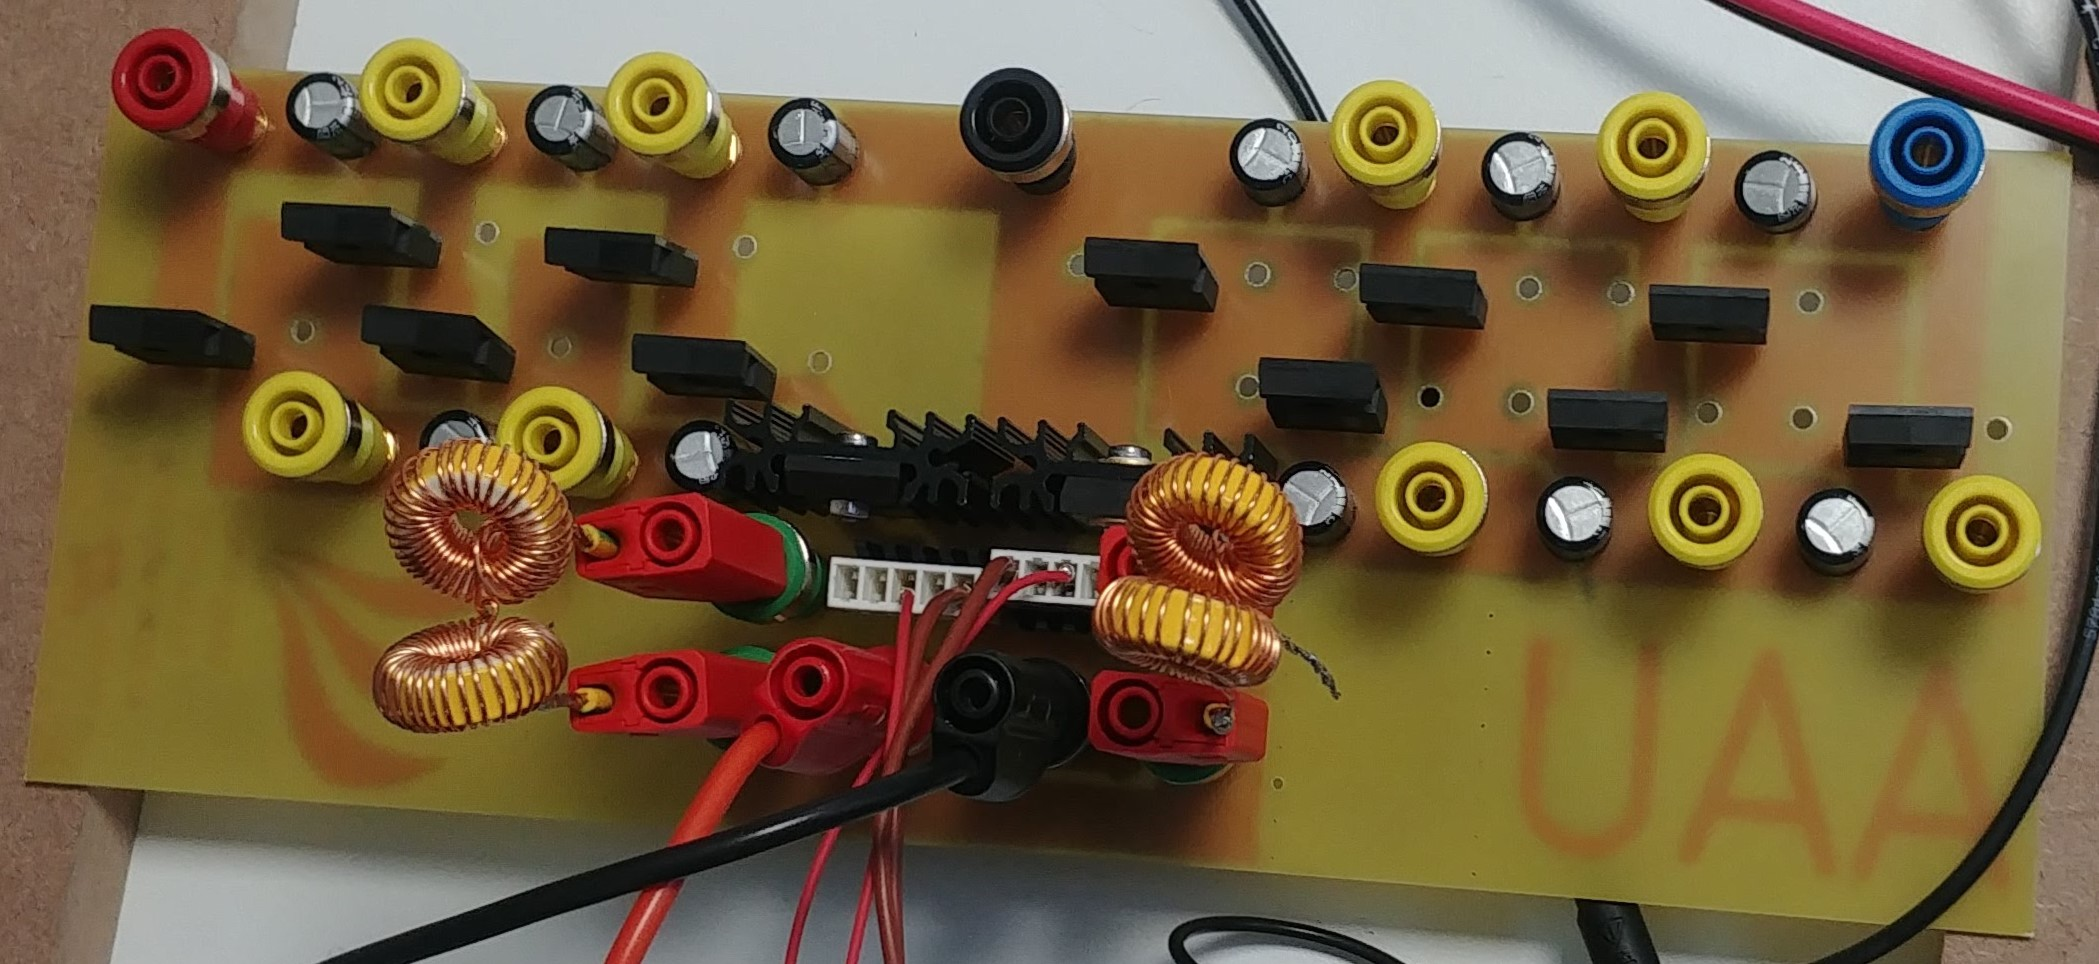
\includegraphics[width=0.8\textwidth]{figures/06Testing/setup.jpg}
	\end{center}
	\vspace{-4mm}
	\caption{PCB with all the components mounted}
	\label{fig:SETUP}
\end{figure}

To generate the PWM input, two wave generators were used, due to the easy synchronisation. The tools used for measurements were Tektronix DPO2024B Oscilloscopes and Keysight 34450A multimeters, all available for us in the AAU Esbjerg laboratories.
All the data presented in the next section has been captured in these devices, results are limited to their accuracy.
\todo {names of scopes} 
\clearpage
\vspace{-6mm}
\section{Results}

After the setup was complete the first test ran, to test the overall output voltage of the topology within the range of possible duty cycles. The purpose of this tests is too see if the expected gain is matched and what part of the differences are expected and what the unexpected ones can be justified by. 
\vspace{-4mm}

\begin{figure}[H]
	\begin{center}
   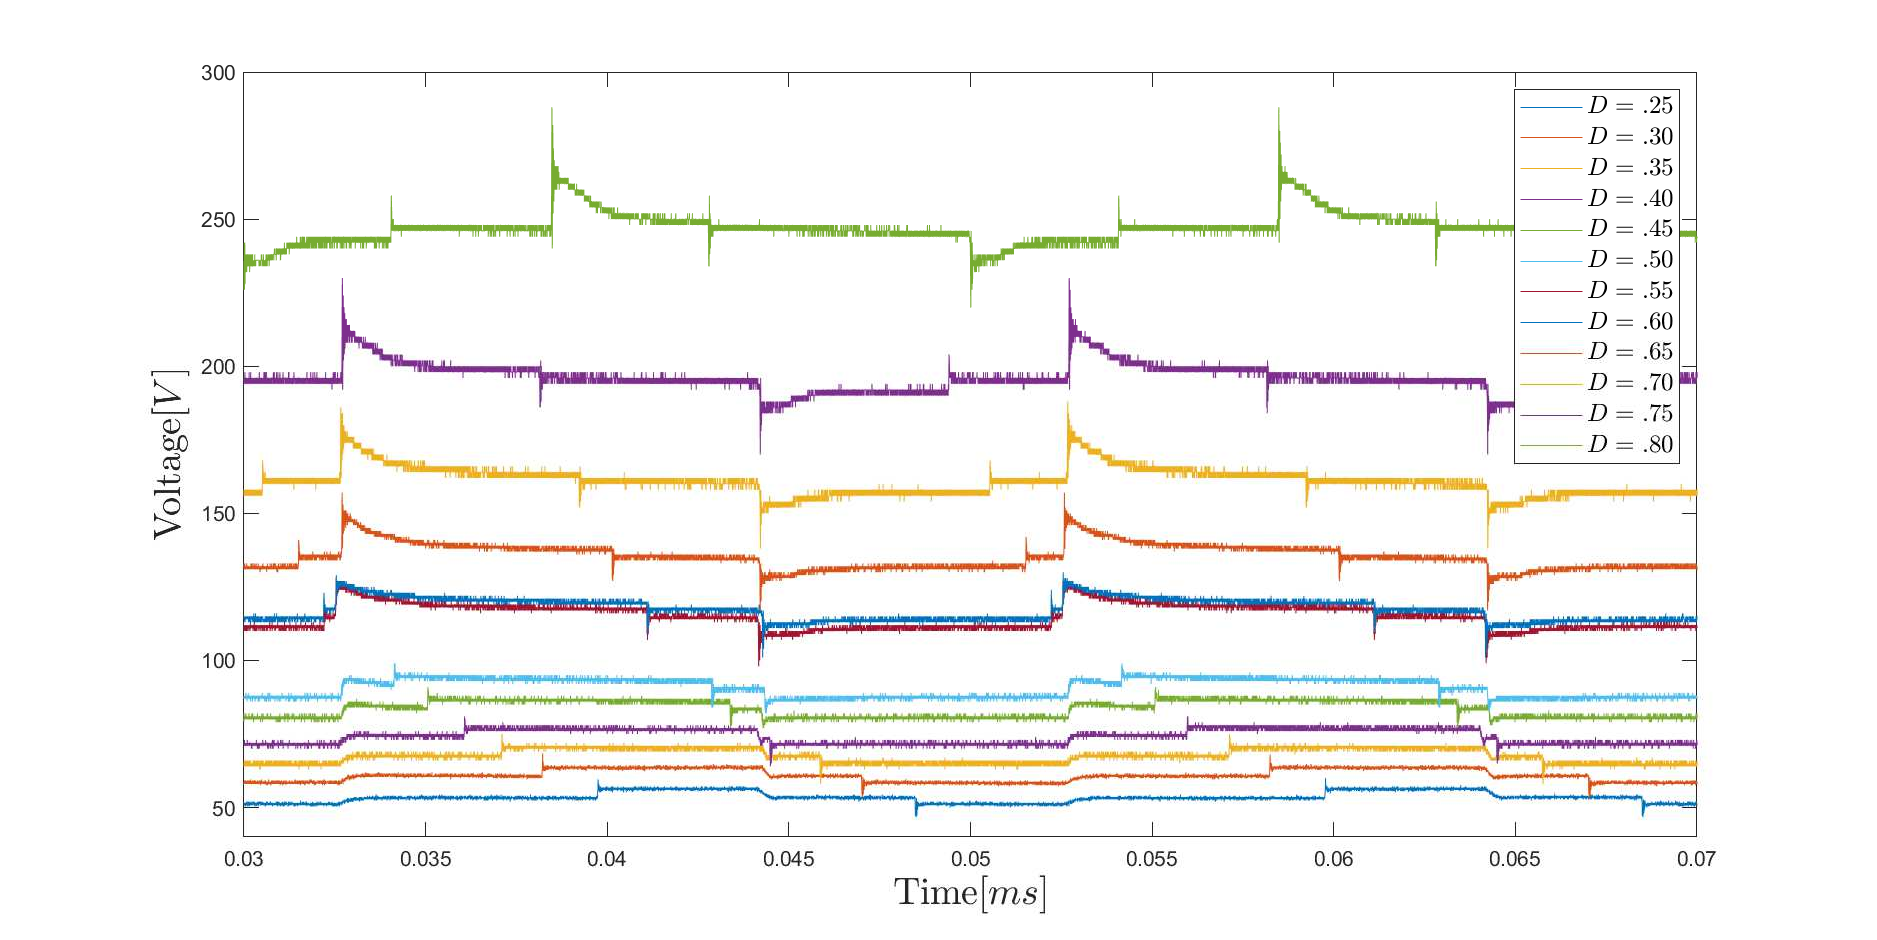
\includegraphics[width=\textwidth]{figures/06Testing/Vripple10Vin.pdf}
	\end{center}
	\vspace{-8mm}
	\caption{$V_o$ at duty cycles between 0.25 and 0.8}
	\label{fig:V_OUT_ALL}
\end{figure}
\vspace{-4mm}
All the output voltage waves can be seen on Fig. \ref{fig:V_OUT_ALL}. To put those values, they need to be compared to the expected values from the expressions we've already derived. All of the calculated and measured values can be seen in the Table \ref{tab:V_OUT_ALL}.
\vspace{-2mm}

\begin{table}[H]
\begin{center}
\caption {Calculated and Measured output voltages} \label{tab:V_OUT_ALL} 
\vspace{-1mm}
\begin{tabular}{|l|l|l|l|}
\cline{1-4}
Duty cycle & Calculated $V_o$ & Measured $V_o$& Difference \\ \cline{1-4}
0.25&	63.9V & 52.6V & 11.3V \\ \cline{1-4}
0.30&	70.0V & 59.7V & 10.3V \\ \cline{1-4}
0.35&	75.9V & 66.1V & 9.8V \\ \cline{1-4}
0.40&	82.9V & 71.8V & 11.1V \\ \cline{1-4}
0.45&	92.2V & 76.4V & 15.7V \\ \cline{1-4}
0.50&	102.4V & 83.3V & 19.1V \\ \cline{1-4}
0.55&	114.9V & 93.1V & 21.8V \\ \cline{1-4}
0.60&	125.0V & 106.8V & 18.2V\\ \cline{1-4}
0.65&	144.3V & 123.9V & 20.4V \\ \cline{1-4}
0.70&	162.4V & 147.0V & 15.4V\\ \cline{1-4}
0.75&	194.2V & 182.5V & 11.7V \\ \cline{1-4}
0.80&	245.8V & 221.0V & 24.8V\\ \cline{1-4}
&	 & Average loss:  & 15.8V \\ \cline{1-4}
\end{tabular}
\end{center}
\end{table}

The results show variable difference in favour of the calculated values. That is completely expected as all of the components apart from the diode and MOSFET were assumed ideal. Internal resistance and power consumption of all components can justify some of the losses. What is less expected is that there is no clear pattern in the decreases, which can be accounted to imperfect measurement or overall inconsistency in the tests and/or equipment. 

To validate our simulation results,
we tested the hardware in depth at a duty ratio $D = 0.6$.
This is the standard we used throughout all simulations described in Chapter \ref{ch:dev}.
We took all measurements possible with our board layout,
which mostly allowed for voltage measurements between components.
The only place where we could measure the current was at the inductors.

Figure \ref{fig:bottopcharge} shows a comparison of the charging components.

\begin{figure}[H]%
    \centering
    \subfloat[Bottom Capacitor Voltages]
    {{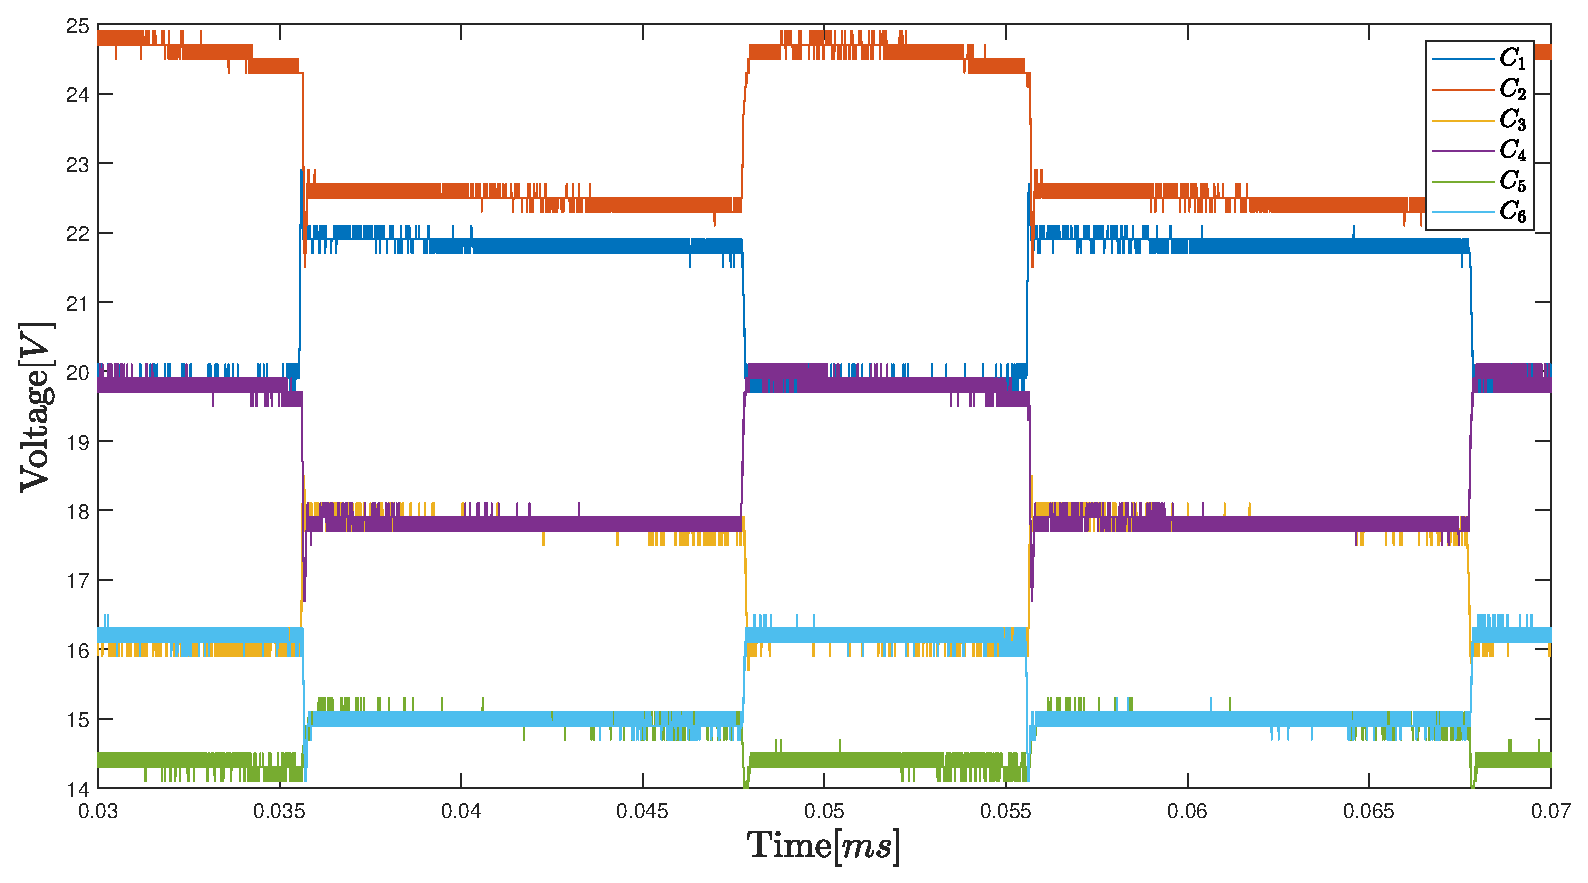
\includegraphics[width=0.5\textwidth]{figures/06Testing/botcap60per.eps} \label{fig:botcap60per}}}%
    \subfloat[Top Capacitor Voltages]
    {{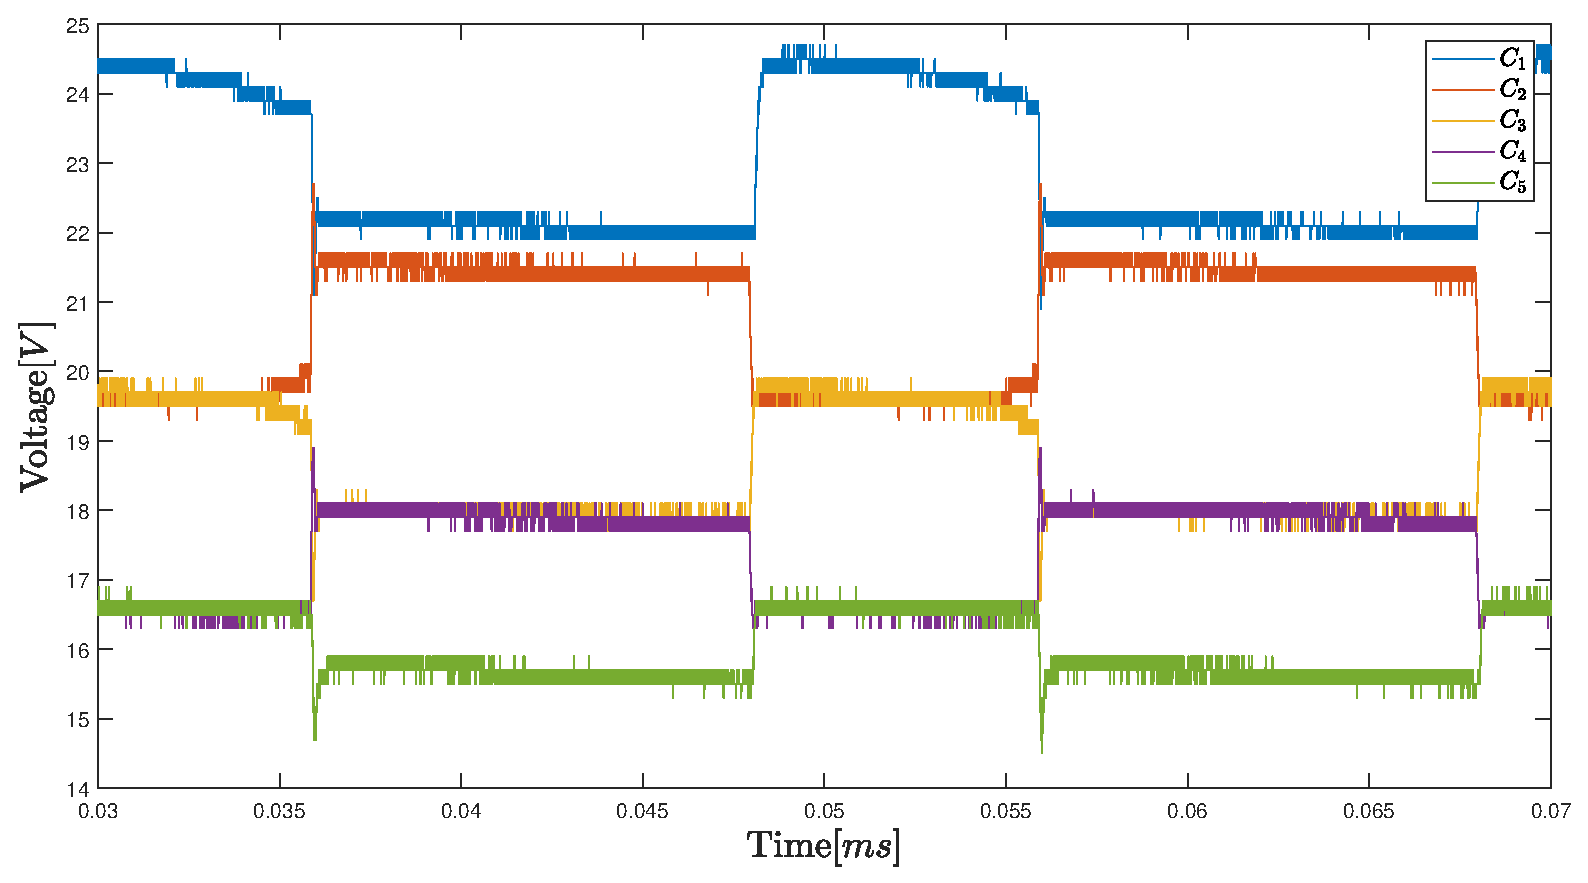
\includegraphics[width=0.5\textwidth]{figures/06Testing/topcap60per.eps} \label{fig:topcap60per}}}%  
   \qquad
    \subfloat[Bottom Inductor Current/Voltage]
    {{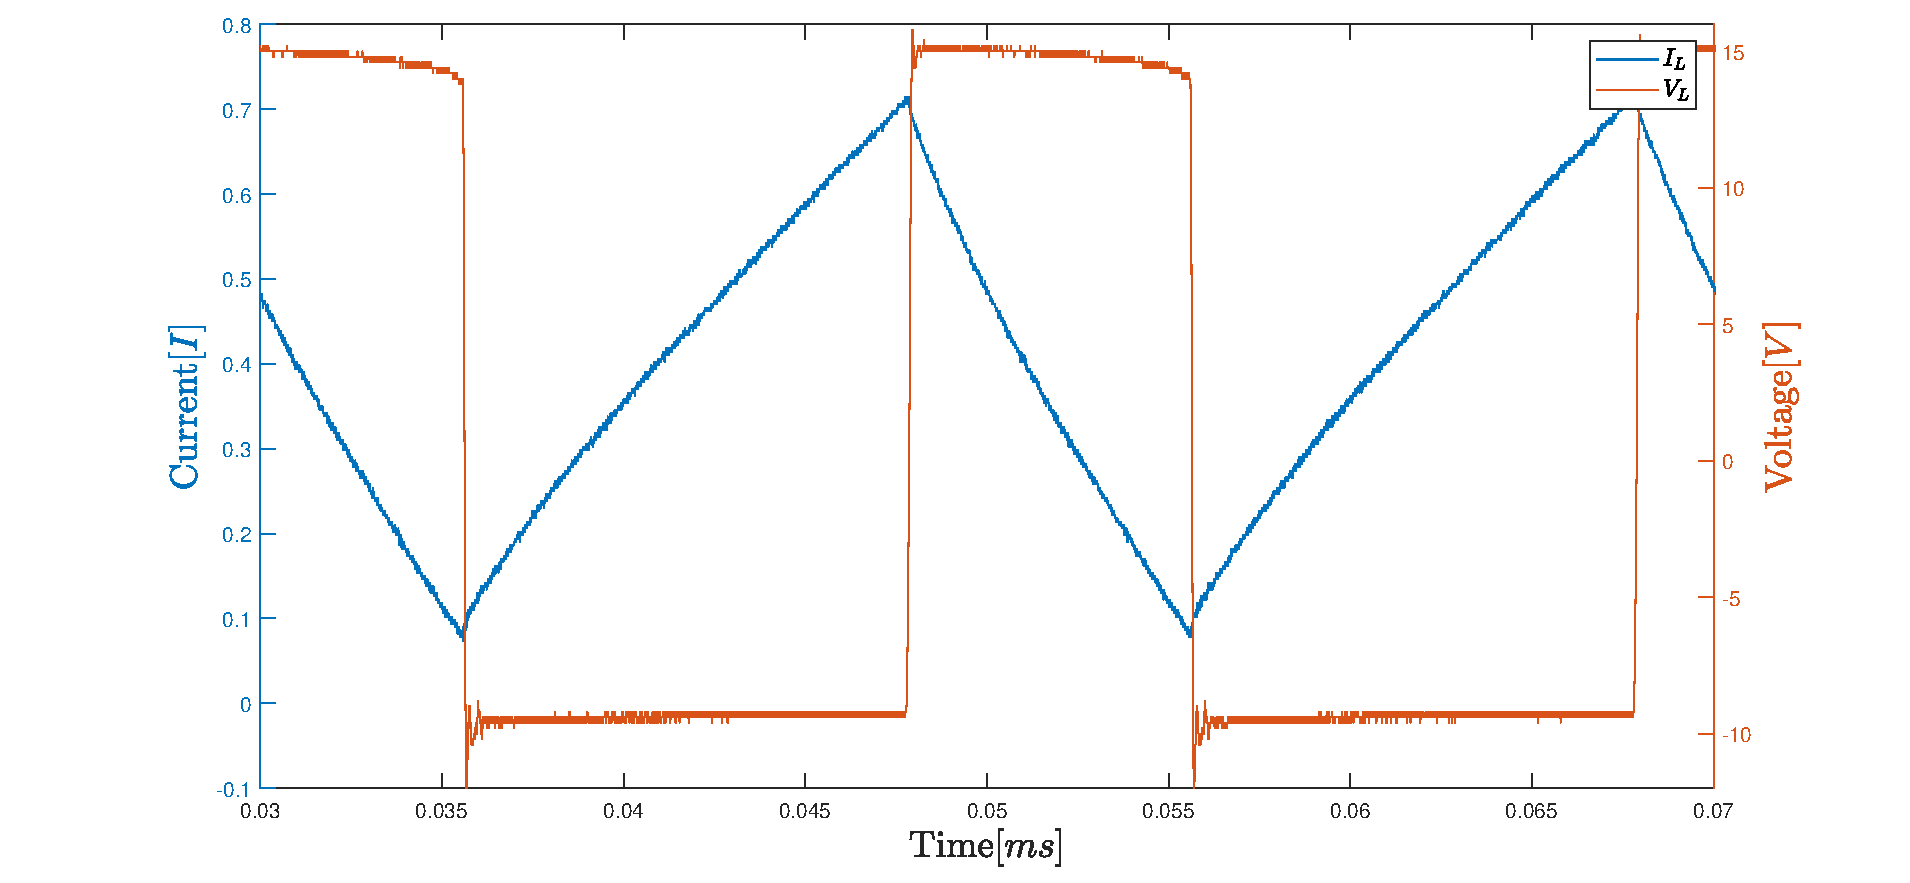
\includegraphics[width=0.5\textwidth]{figures/06Testing/botind60per.eps} \label{fig:botind60per}}}%
    \subfloat[Top Inductor Current/Voltage]
    {{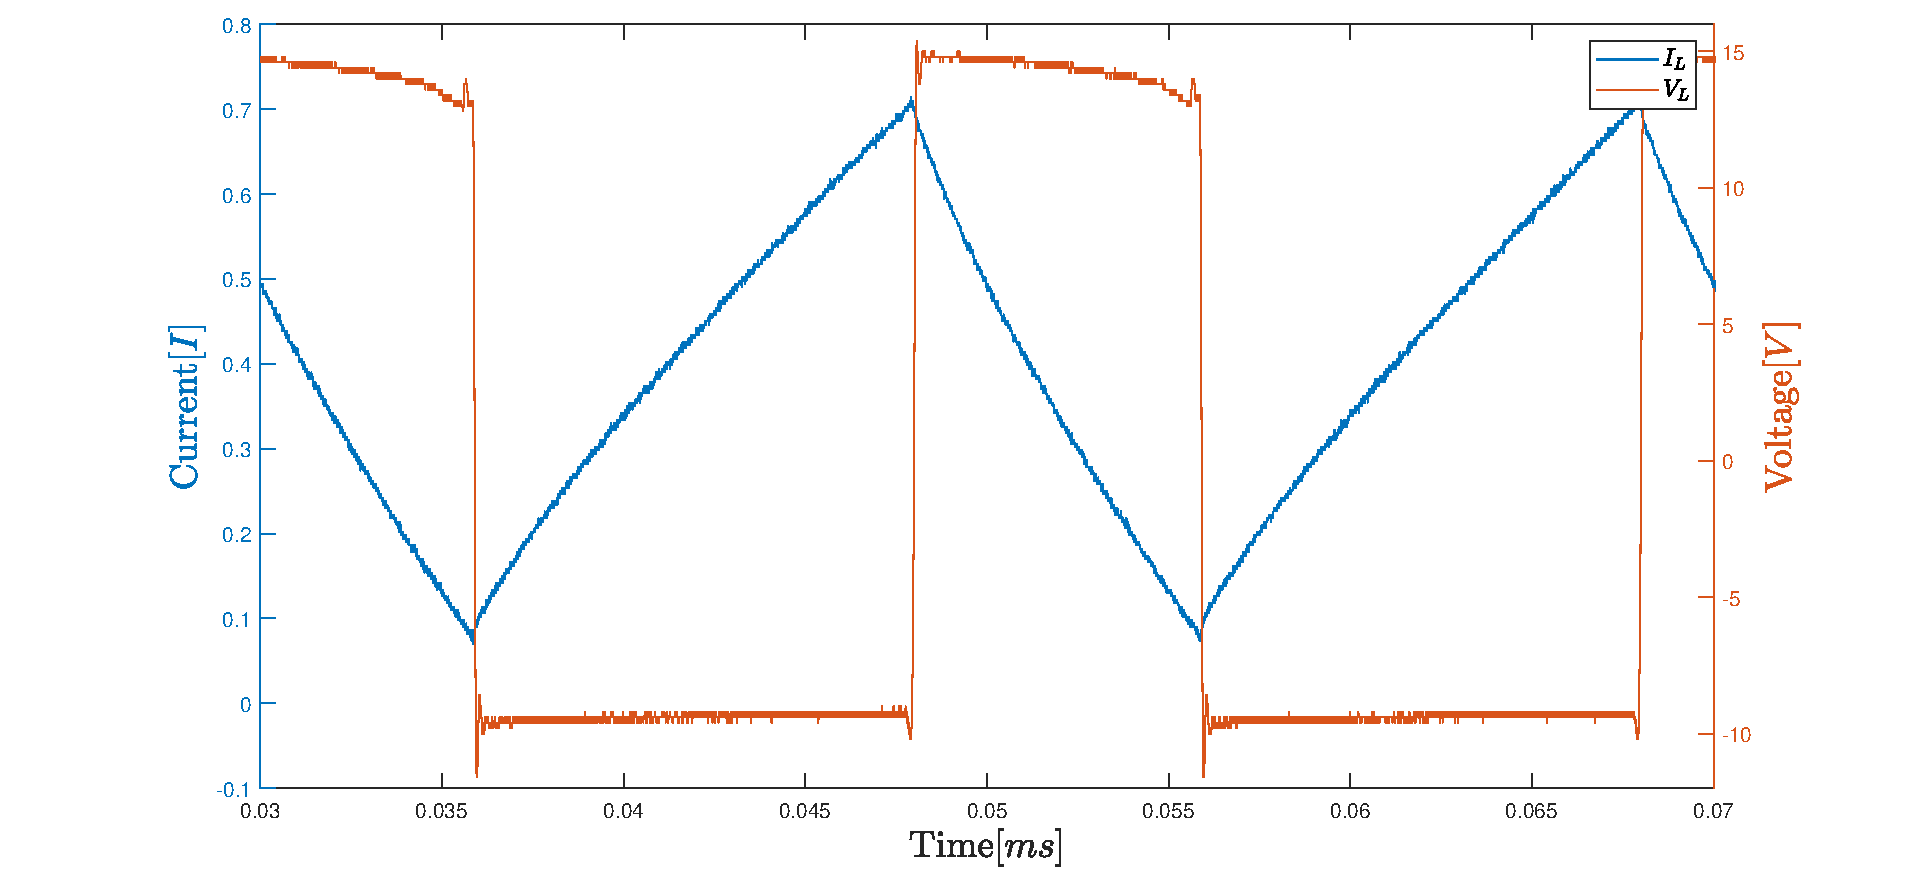
\includegraphics[width=0.5\textwidth]{figures/06Testing/topind60per.eps} \label{fig:topind60per}}}%  
    \caption{Bottom/Top Comparison of Charging Components}%
     \label{fig:bottopcharge}%
\end{figure}
\todo{put figures in appendix}

To be noted is that the bottom (\ref{fig:botcap60per}) is an inverting NxBC,
while the top is non inverting.
Because of that the naming of the capacitors varies slightly.
For simplicity,
we will from now on only talk about the top measurements (visible on the right).

It can be observed that the capacitor voltage $V_{C_1}$ is higher than the other voltages,
as expected in Chapter \ref{ch:dev}.
Also the voltage across this capacitor fits perfectly to the simulations,
with a mean of $23.5 V$.
The subsequent capacitors all have a falling voltage,
compared to the previous,
which suggests that our drop calculation is correct.
The amount of drop between the stages is higher than in the simulations,
which we expected,
because we used ideal components to simulate capacitors and inductors.

The repetitive charging and discharging heats both inductors and capacitors up,
which was not included in the simulations.
Also the internal resistance was neglected in the simulations.
The drops between the stages,
suggests a limited amount of stages to be beneficial.
This is a commonly known problem with the Cockcroft-Walton Multiplier.


Investigating the inductors current and voltage (\ref{fig:botind60per} \& \ref{fig:topind60per}),
we can observe that the converter is in continuous conduction mode (CCM) at $D = 0.6$.
There is even the option to go to a lower $D$,
as the current doesn't reach $0 A$.
The current is very low in total,
because $R_L$ was chosen very big.

The voltage across the inductors can be observed to have a range from $-10 V$ to $15V$.
The negative offset is observed because the negative measuring point is directly connected to $V_{IN} +$
The total range of the inductor voltage is $25V$, which is also the highest $C_{1}$ charges up to.





\begin{figure}[H]%
    \centering
    \subfloat[Bottom Diode Voltages]
    {{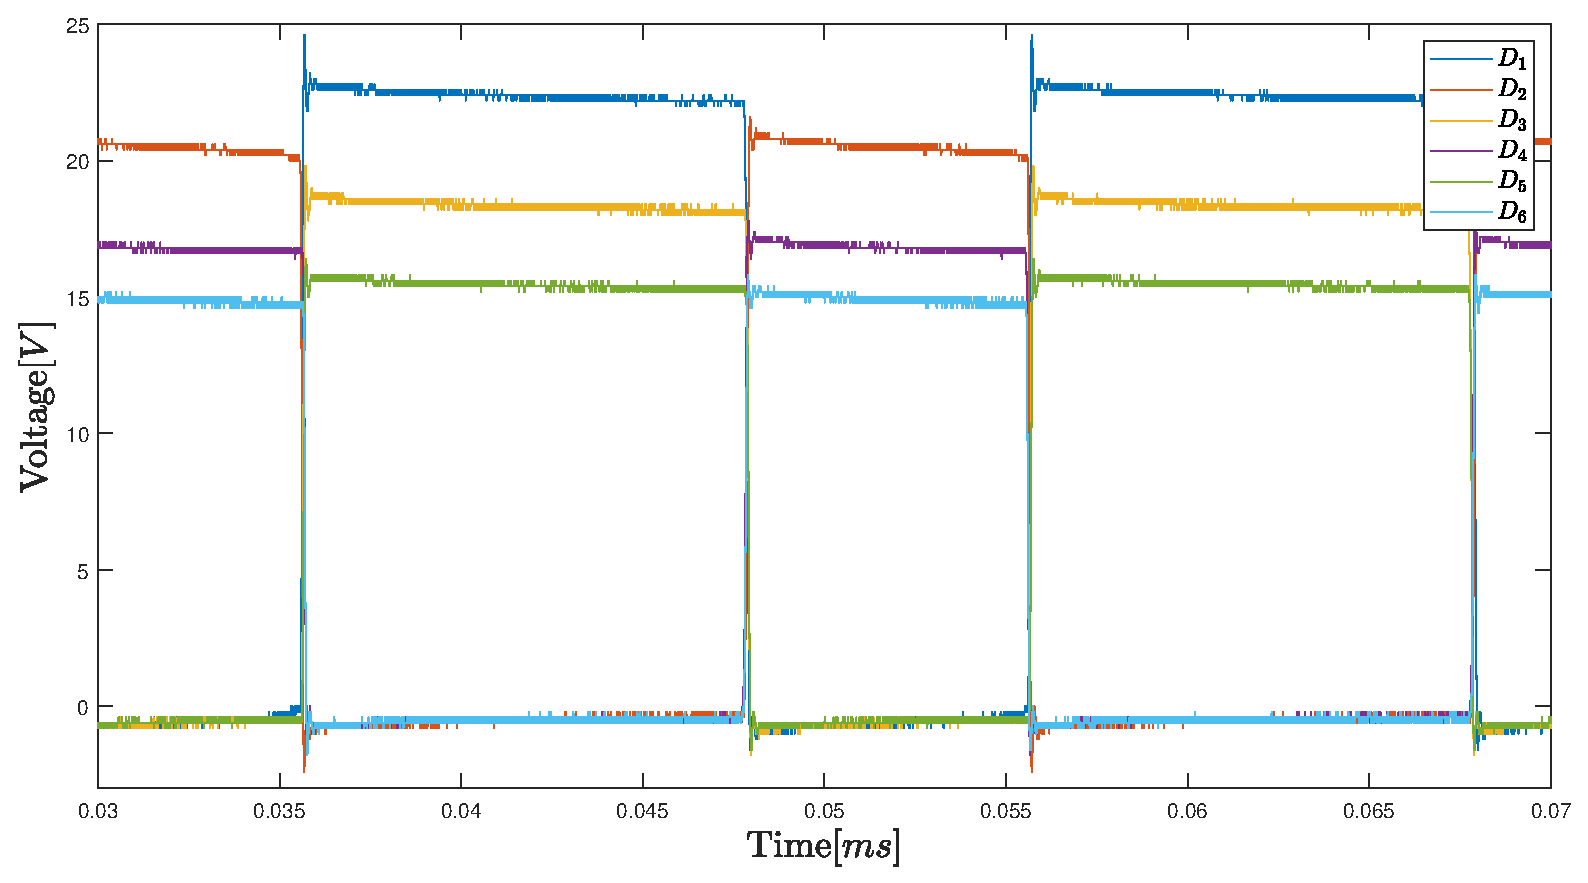
\includegraphics[width=0.5\textwidth]{figures/06Testing/botdio60per.eps} \label{fig:botdio60per}}}%
    \subfloat[Top Diode Voltages]
    {{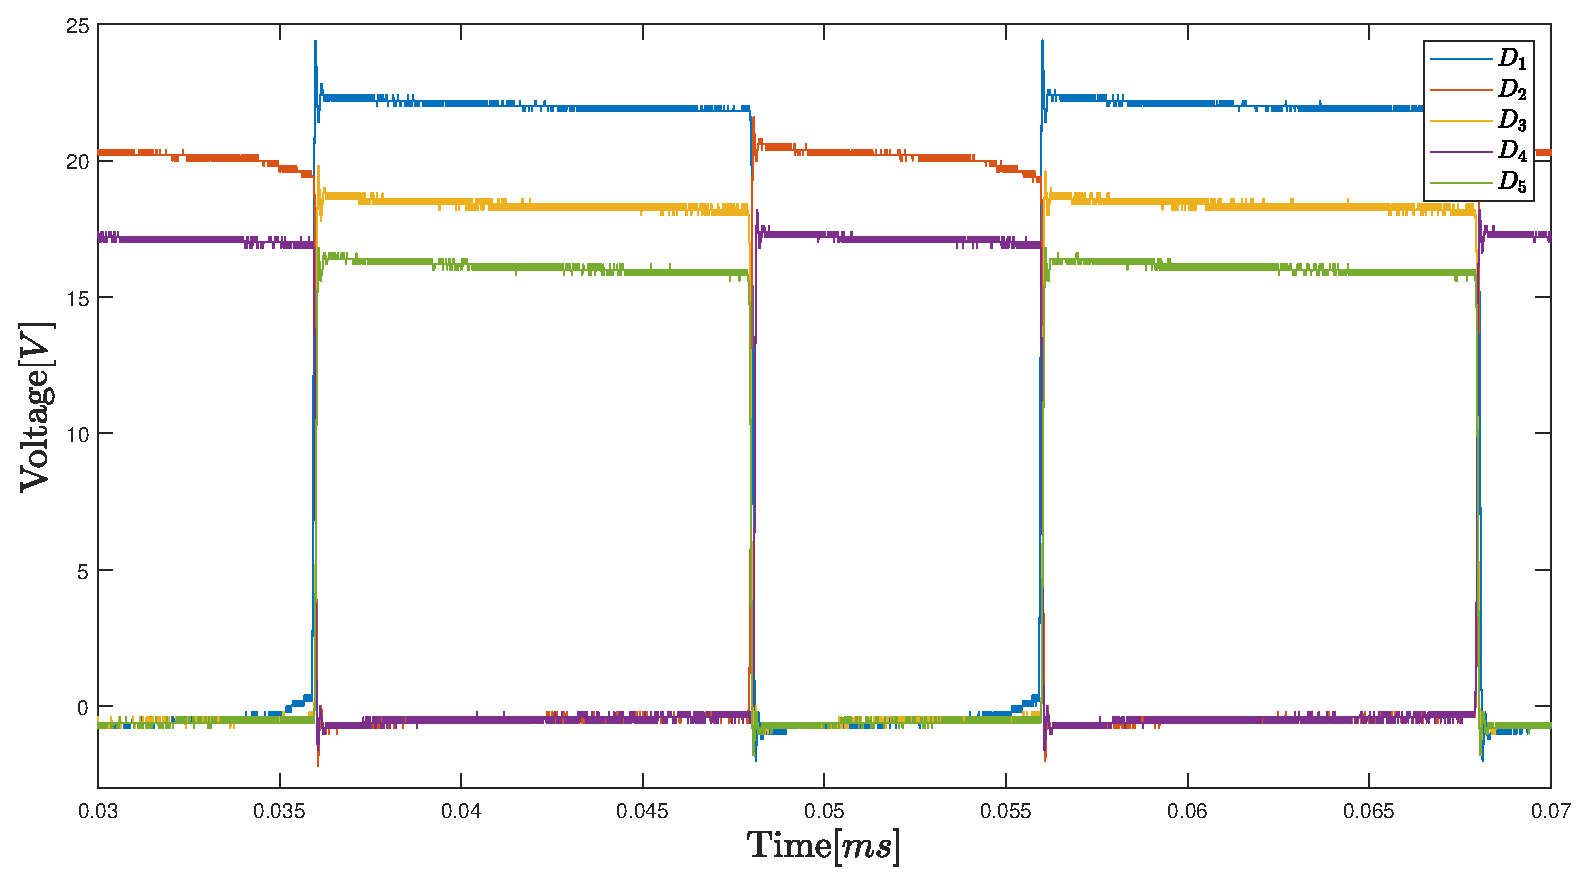
\includegraphics[width=0.5\textwidth]{figures/06Testing/topdio60per.eps} \label{fig:topcap60per}}}%  
   \qquad
    \subfloat[Bottom MOSFET Current/Voltage]
    {{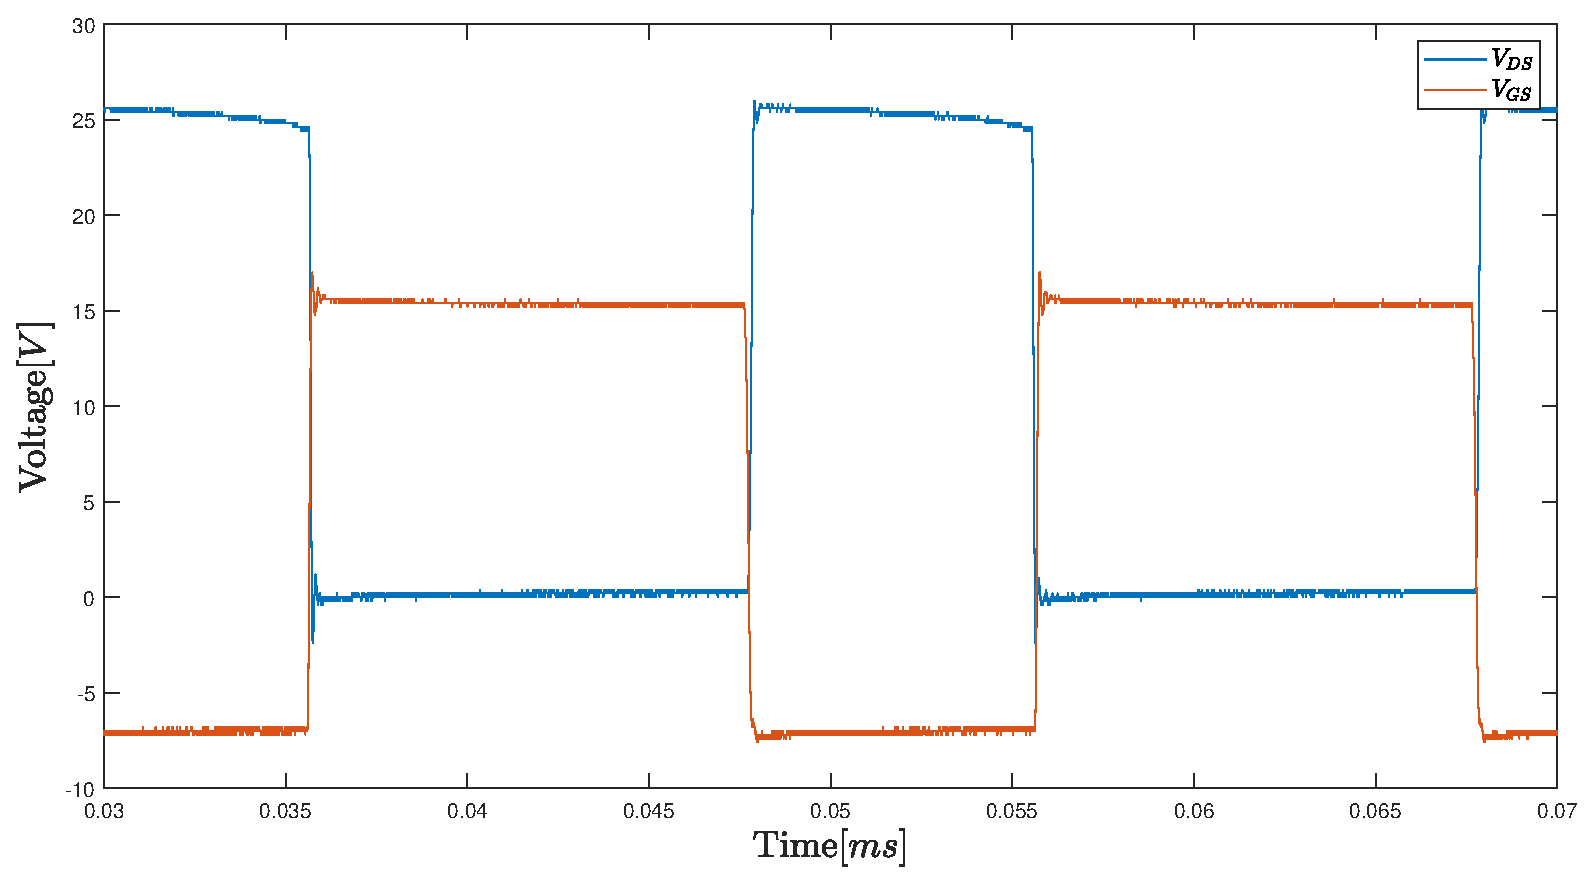
\includegraphics[width=0.5\textwidth]{figures/06Testing/botswi60per.eps} \label{fig:botind60per}}}%
    \subfloat[Top MOSFET Current/Voltage]
    {{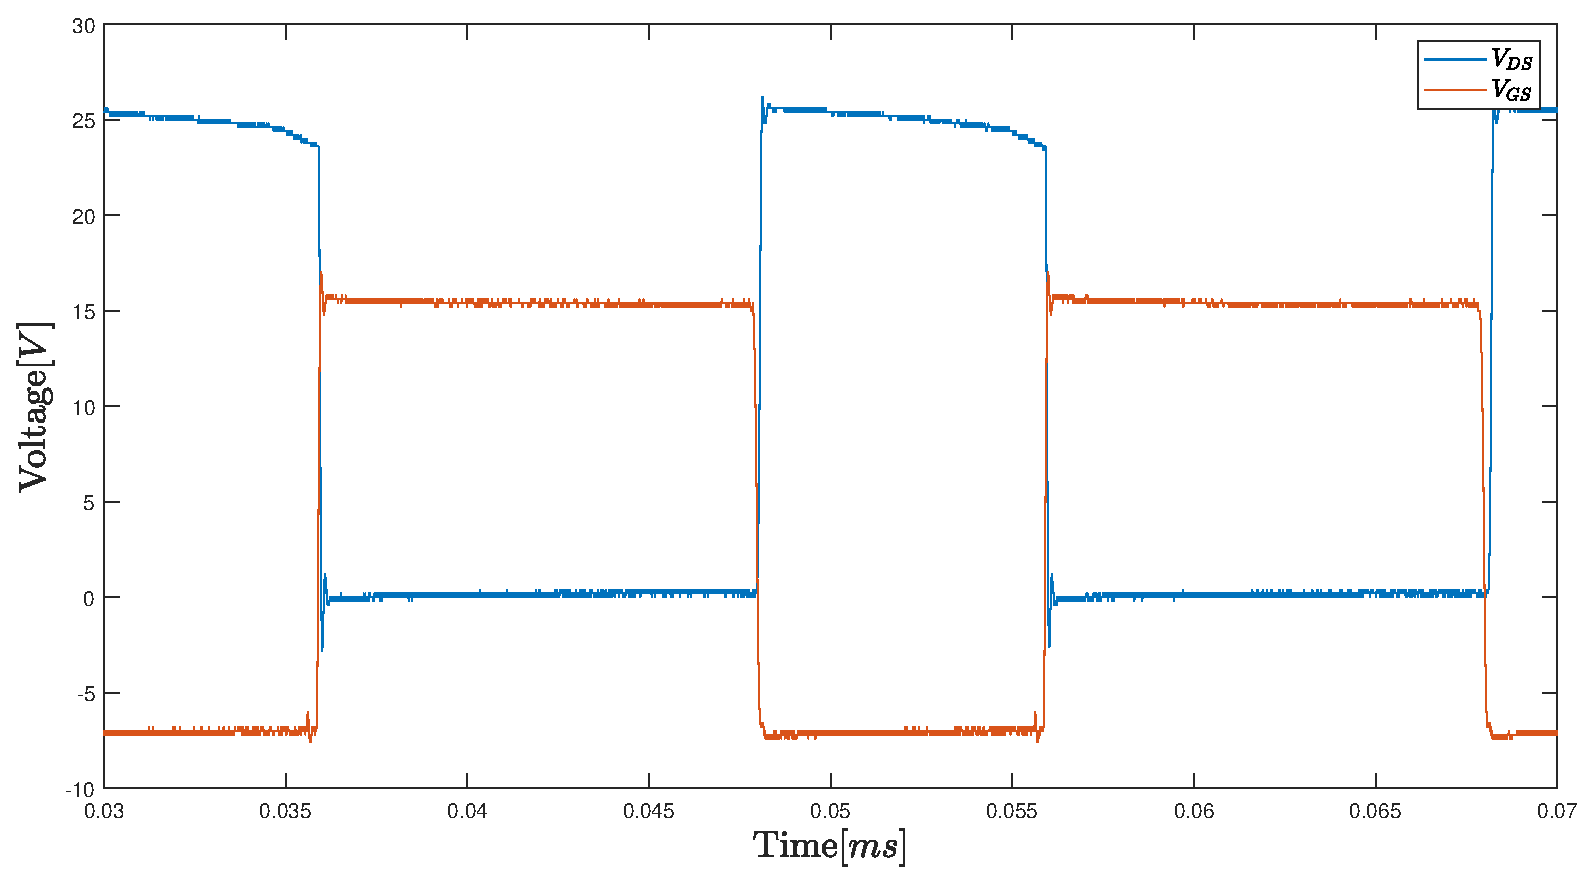
\includegraphics[width=0.5\textwidth]{figures/06Testing/topswi60per.eps} \label{fig:topind60per}}}%  
    \caption{Bottom/Top Comparison of Switching Components}%
     \label{fig:bottopswitch}%
\end{figure}
\todo{put figures in appendix}

The plot on Figure \ref{fig:bottopswitch} show the voltages across the diodes and across the terminals of the MOSFET.
The voltage levels over the diode confirm the statement already made about the capacitors - the voltage decreases over the higher levels of the circuit.
Another significant observation is that the negative voltage level is relatively consistent over the circuit, which improves the validity of the calculations in Section. \ref{ch:DROPS}.

The first conclusion we can draw from the MOSFET graphs is that the levels of $V{GS}$ confirm our switching circuit. 
The fact that the level are equal to the ones coming from the SKYPER board and the duty cycle is as expected proves that. 
The second major observation is that the stress over the switch $V{DS}$ during OFF state is equal to that of a CBC. 
This means that the requirements for a MOSFET for this topology are the same as the ones for a CBC, while the gain is higher.

To measure the efficiency of the converter the power on the input and output was measured.
This was done by taking the current from the source at a constant voltage and the current through the load, which size was known. So the powers and efficiency can be calculated.

% Pin = Vin*Iin Pout = I^2*R
\begin{equation}
	P_{in}= V_{in} \times I_{in}
	\label{eq:EfficiencyPin}
\end{equation}

\begin{equation}
	P_{out}= I_{out}^2 \times R_{load}
	\label{eq:EfficiencyPout}
\end{equation}

\begin{equation}
	\eta = (\frac{P_{out}}{P_{in}})
	\label{eq:Efficiency}
\end{equation}


The measured efficiency for different duty ratios can be found in the table below.

\begin{table}[H]
\begin{center}
\caption {Efficiency of the converter} \label{tab:Efficiencyandpowers} 
\vspace{-1mm}
\begin{tabular}{|l|l|l|l|l|l|l|}
\cline{1-7}
Duty cycle & $V_{in}$ & $I_{in}$ & $I_{out}$ & $P_{in}$	& $P_{out}$ & Efficiency \\ \cline{1-7}
0.25 &	10.00V &	0.215A &	0.021A &	2.15W &	1.11W &	51.77\% \\ \cline{1-7}
0.30 &	10.00V &	0.266A &	0.024A &	2.66W &	1.44W &	54.14\% \\ \cline{1-7}
0.35 &	10.00V &	0.318A &	0.027A &	3.18W &	1.82W &	57.31\% \\ \cline{1-7}
0.40 &	10.00V &	0.368A &	0.029A &	3.68W &	2.10W &	57.13\% \\ \cline{1-7}
0.45 &	10.00V &	0.409A &	0.031A &	4.09W &	2.40W &	58.74\% \\ \cline{1-7}
0.50 &	10.00V &	0.480A &	0.034A &	4.80W &	2.89W &	60.21\% \\ \cline{1-7}
0.55 &	10.00V &	0.587A &	0.038A &	5.87W &	3.61W &	61.50\% \\ \cline{1-7}
0.60 &	10.00V &	0.759A &	0.043A &	7.59W &	4.62W &	60.90\% \\ \cline{1-7}
0.65 &	10.00V &	1.000A &	0.050A &	10.00W &6.25W &	62.50\% \\ \cline{1-7}
0.70 &	10.00V &	1.381A &	0.059A &	13.81W &8.70W &	63.02\% \\ \cline{1-7}
0.75 &	10.00V &	2.092A &	0.073A &	20.92W &13.32W&	63.68\% \\ \cline{1-7}
0.80 &	10.00V &	3.095A &	0.088A &	30.95W &19.36W&	62.55\% \\ \cline{1-7}
\end{tabular}
\end{center}
\end{table}
